%% notes-tex/multimodal/043-datasets-primer/sections/input-design.tex
%% SOURCE: torchcell/datamodels/schema.py (genotype classes); results/store_census.json and
%% results/data_shapes_043.json (counts per record, slurm job 5902); results/distinct_alleles.json
%% (experiments/043-expression-proteome-morphology/scripts/count_distinct_alleles.py, one pass
%% over allReferenceGenesWithSNPsAndIndelsInferred.tar.gz); the genomes tier
%% ($DATA_ROOT/torchcell-genomes/peter2018_1011_assemblies/manifest.json); the stored S288C
%% embedding tables under $DATA_ROOT/data/scerevisiae/*_embedding/processed; main's
%% experiments/embeddings/compute_isolate_embeddings.py and
%% experiments/embeddings/results/poc_isolate_fudt_feasibility.json; the retrospective
%% branch's notes-tex/perturbation-operator and torchcell/models/equivariant_cell_graph_transformer.py;
%% experiments/019-simb-multimodal/conf/train_cgt_multitask.yaml; the mirrored Peter 2018
%% paper and SI (peter1011GenomeEvolution2018). Prototype: torchcell/models/genotype_tokens_043.py.
%% Design decisions of the 2026-10-20 review pass (representation reviewer, reconciled by
%% the driver); code follows in the next stage.

\section{The input side: sequence, genotype and the perturbed cell graph\secstatus{todo}}
\label{sec:input}

Five genotype classes have to enter one model so that every gene-level readout trains
together: engineered deletions and double deletions, natural isolates, segregants and
promoter variants, and the same input has to hold a gene the training set never saw: an
isolate allele, an accessory ORF, a heterologous cassette, a gene of another host. That
constraint fixes the abstraction between the stored genotype and the perturbation
operator: a \term{gene token} per gene from a frozen composite sequence encoder, never
from an identity table; a \term{reference context} per distinct genome (S288C, each
natural isolate, each segregant parent), encoded once and cached; a \term{change type}
per gene per strain that says how the strain's copy differs from its reference; a
\term{position} term carrying chromosome, relative coordinate and copy number; and
\term{context tokens} for what is true of the record rather than of a gene, which the
heads read (Sec.~\ref{sec:output-tokens}). The perturbation operator then reads the
strain's engineered edits exactly as it reads deleted genes today. Everything measured
below is read off the 043 store census, the shape pass, the genomes tier or the stored
embedding tables; what is proposed is marked as such, and the decisions collected in
Sec.~\ref{sec:input-decisions} carry one recommended option each.
Table~\ref{tab:input-symbols} defines the symbols and Fig.~\ref{fig:input-side} draws the
path.

%% SOURCE: hand-authored definitions; the widths are those of the 1,084,619-parameter
%% expression model (perturbation-operator document, tab:symbols) and of the stored
%% embedding tables.
\begin{table}[htbp]
\centering
\footnotesize
\caption[]{\textbf{Symbols of the input side}, alphabetical. Widths are those of the
1{,}084{,}619-parameter expression model of experiment 019 (\file{conf/cgt_expr_012.yaml}:
$d=90$, $h=9$ heads) and of the stored S288C embedding tables.}
\label{tab:input-symbols}
\begin{tabular}{>{\raggedright\arraybackslash}p{34mm}>{\raggedright\arraybackslash}p{136mm}}
\toprule
Symbol & Meaning \\
\midrule
$a_i\in\mathcal{A}$ & allele parent of gene $i$ in a segregant: the parent whose block
covers the gene; $\varnothing$ for every other gene and every other genotype class \\
$B$ & strains in a batch \\
$c_i\in\mathcal{C}$ & change type of gene $i$ under the strain's genotype
(Table~\ref{tab:change-types}); $\mathrm{ref}$ when the strain carries the reference copy \\
$\mathcal{C}$ & the change-type vocabulary, seven members \\
$d$ & width of a gene token and of a gene state, 90 \\
$E\in\mathbb{R}^{(|G|+1)\times d}$ & encoder output over the reference cell graph: row 0
the CLS state $h$, rows $1$ to $|G|$ the wild-type gene states $h_i$ \\
$f_k:\Sigma^*\to\mathbb{R}^{d_k}$ & the four frozen sequence encoders of the composite
token, $k\in\{\mathrm{up},\mathrm{down},\mathrm{prot},\mathrm{cds}\}$: FUDT upstream (768),
FUDT downstream (768), ProtT5 (1{,}024), CaLM (768) \\
$G^{(s)}$ & the gene set of reference context $s$; $|G^{(\mathrm{S288C})}|=6{,}607$, written
$G$ where the context is S288C \\
$H\in\mathbb{R}^{B\times|G|\times d}$ & perturbed gene states, the operator's output
(\file{H_genes_pert}) \\
$h,\;h^{\mathrm{pert}}\in\mathbb{R}^{d}$ & the CLS state before and after the operator \\
$M$ & marked genes of a strain, $M=\sum_i m_i$; the operator's key count \\
$m\in\{0,1\}^{|G|}$ & the mark: $m_i=\mathbf{1}[c_i\neq\mathrm{ref}]$ \\
$P_i\in\mathbb{R}^{d}$ & the position term of gene $i$ (Eq.~\ref{eq:input-position}) \\
$\mathbf{p}_t\in\mathbb{R}^{d}$ & token of the $t$-th marked gene, the operator's key
and value source \\
$\pi_i=(\chi_i,\rho_i,\kappa_i)$ & position of gene $i$: chromosome index
$\chi_i\in\{0,\dots,16\}$ (0 the mitochondrion), relative reference coordinate
$\rho_i=\tfrac{1}{2}(\mathrm{start}_i+\mathrm{end}_i)/L_{\chi_i}$, pangenome copy number
$\kappa_i$ \\
$s_i(\gamma)\in\Sigma^*$ & realized sequence of gene $i$ under genotype $\gamma$ \\
$T\in\mathbb{R}^{|\mathcal{C}|\times d}$, $A\in\mathbb{R}^{|\mathcal{A}|\times d}$ &
learned change-type and allele-parent embeddings; $T_{\mathrm{ref}}=A_{\varnothing}=0$ \\
$t_{\mathrm{type}},\;t_{\mathrm{env}}$ & the ontology-path and environment tokens, read
by the heads (Sec.~\ref{sec:output-tokens}); the dataset enters only as the per-dataset
bias at the head \\
$X^{(s)}\in\mathbb{R}^{|G^{(s)}|\times d}$ & gene tokens of reference context $s$, computed
once and cached; $X=X^{(\mathrm{S288C})}$ \\
$\tilde X\in\mathbb{R}^{B\times|G|\times d}$ & realized gene tokens of a batch,
$\tilde X_{b,i}=X_i+T_{c_{b,i}}+A_{a_{b,i}}$ \\
$z_S\in\mathbb{R}^{d}$ & pool over a strain's marked rows of $H$ (\file{pooled_perturbed}) \\
\bottomrule
\end{tabular}
\end{table}

\subsection{What enters the model today\secstatus{todo}}
\label{sec:input-today}

The 019 expression model builds its gene tokens from a learned table, not from
sequence: \file{conf/train_cgt_multitask.yaml} sets \file{node_embeddings: []} and
\file{learnable_embedding.enabled: true}, so $X$ is an \file{nn.Embedding(6607, d)}
indexed by gene order, and the CLS row is one learned vector shared by every strain. The
encoder runs once per step on the wild-type graph; a strain enters only through the
operator, whose token for a deleted gene is that gene's encoder state,
$\mathbf{p}_t=h_{g(t)}$. The Methods write $\mathbf{p}_t=r(e_t)+\mathbf{t}_{\tau_t}+m_t\mathbf{w}$
with a perturbation-type embedding $\mathbf{t}_\tau$; the code implements neither the type
term nor the magnitude term (perturbation-operator document, Table of symbols). Three
consequences for the 043 classes are measured:
\begin{itemize}
\item A deletion and any other mark on the same gene produce the same key and the same
value, since the token is the gene state alone.
\item The \texttt{Perturbation} processor marks every perturbation of a record, so a
Caudal isolate enters with 5{,}575 of 6{,}607 genes in \file{pert_mask}
(Sec.~\ref{sec:genotypes}), and under operator A their 5{,}575 values are averaged into
one vector delivered to every gene.
\item A segregant enters with \file{pert_mask} all false and is the reference strain.
\end{itemize}
The sequence encoders exist on \file{main} and are already keyed by gene:
\file{NodeEmbeddingBuilder} serves ProtT5 on the protein (\file{prot_t5_xl_uniref50}),
nucleotide-transformer windows of 5{,}979 bp around the ORF and of 1{,}003 bp upstream and
300 bp downstream, the fungal up-down transformer on the upstream and downstream
flanks, CaLM and codon frequency on the coding sequence, and one-hot identity. Each is
one frozen row per reference gene, concatenated into \file{cell_graph["gene"].x} and
projected by the model's preprocessor. None of them has a per-strain version.

\subsection{The gene token\secstatus{todo}}
\label{sec:input-token}

\notesec{Definition} Gene $i$'s token is the composite of four frozen sequence encoders on
its realized sequence under reference context $s$, each block standardized and projected,
plus the position term of Sec.~\ref{sec:input-position}:
\begin{equation}
X^{(s)}_i=\sum_{k\in\{\mathrm{up},\mathrm{down},\mathrm{prot},\mathrm{cds}\}}
W_k\,\operatorname{LN}_k\!\big(f_k(s^{k}_i)\big)\;+\;P_i,
\qquad W_k\in\mathbb{R}^{d\times d_k},
\label{eq:input-composite}
\end{equation}
with $f_{\mathrm{up}}$ the fungal up-down transformer (FUDT) on the 1{,}003 bp window
ending at the start codon, $f_{\mathrm{down}}$ its downstream model on the 300 bp window
from the stop codon, $f_{\mathrm{prot}}$ ProtT5-XL on the protein and $f_{\mathrm{cds}}$
CaLM on the codon sequence; the widths are those of the stored S288C tables (768, 768,
1{,}024, 768; \file{data/scerevisiae/\{fudt,protT5,calm\}\_embedding/processed}). Each
block has its own layer normalization, so a 1{,}024-wide block does not outweigh a 768-wide
one, and its own projection, so one block can be swapped without retraining the others.
This is the composite of experiments 030 and 031 (\file{--node-embeddings fudt\_upstream
fudt\_downstream prot\_T5\_all calm}); on betaxanthin it reads 0.219 against ProtT5 alone
at 0.216 (031 rounds 232 and 233), and in the trigenic per-entry-token run it reaches a
validation interaction Pearson of 0.5655 (seed 0, epochs 164 to 181, random split). The
encoders are frozen: the 031 operator audit found the single-deletion score to be a
learned affine read of the deleted gene's own sequence token, and nothing measured says
fine-tuning a 1.2-billion-parameter encoder on 1{,}482 deletion profiles would help. The
projections $W_k$, the change-type table $T$ and the position term are the trained part.

A learned identity table is not an option for the base token: a one-hot row is not a
function of sequence and cannot produce a token for an isolate allele, an accessory ORF, a
heterologous cassette or a gene of another host. It survives as one ablation arm, the
transductive ceiling of gene identity on splits A and B, which measures what the composite
loses by not memorizing the gene and enters no claim.

\notesec{Alternatives} Nucleotide-transformer windows (2{,}560 wide, five-prime 1{,}003 bp
and three-prime 300 bp, both stored) in place of the two FUDT blocks, for a host with no
FUDT species token; FUDT is a species-aware fungal model and covers no bacterium, so one
043 arm carries the swap and compares the two families on yeast before a host change forces
it. ESM2 650M in place of ProtT5, on cost alone: on betaxanthin adding it read 0.216 against
0.219 (031 round 233), and it embeds at about a third of ProtT5-XL's cost, which matters
for the isolate pass of Sec.~\ref{sec:input-embeddings}.

\notesec{A gene unseen in training} gets its token by the same four functions: protein
from its CDS, the two windows from the flanks it sits between. For an isolate allele the
CDS is a member of the gene-keyed tarball and the flanks come from the isolate's own
assembly (Sec.~\ref{sec:input-isolates}); for an accessory ORF the CDS is in
\file{allORFs\_pangenome.fasta.gz} (7{,}796 ORFs); for a heterologous cassette the flanks
are the cassette's promoter and terminator; for \textit{P.~kudriavzevii} the tier already
holds \file{proteins.faa}, \file{cds.fna}, the GFF3 and the FASTA.

\notesec{Deleted gene: the row stays, marked} The deleted gene's row is neither removed
from $X$ nor zeroed. Removing it is the token-edit design, which costs one encoder pass
per strain because the gene set then differs by strain
(\file{notes-tex/perturbation-operator}, Sec.~4); the 019 configuration pays the encoder
once per step and that is the dominant cost it was tuned around (\file{cgt_expr_012.yaml}
header). Zeroing it before the encoder has the same cost and a second defect: a zero row
through layer normalization is the normalized bias, one constant vector, so every
deleted gene becomes the same token and the identity of what was deleted is lost before
the first attention layer. The row therefore keeps its reference token and the deletion
is carried by the change type, $c_i=\mathrm{del}$, which the operator reads as a
learned vector added to the token (Sec.~\ref{sec:input-operator}). The gene's own
readout entry is then predicted from a token that says ``this gene, deleted'', which
is the information the deleted-gene flag $\delta_{i,t}$ of the perturbation-operator
document supplies; the predicted $+0.036$ against a measured $-2.42$ for that entry is
what the flag, and now the mark, exists to fix.

\notesec{Variant gene: the allele's own token} For a natural isolate every
\texttt{SequenceVariantPerturbation} points at the isolate's allele through a
sha256-pinned \file{sequence\_ref}, so $f_k$ is computable on the allele for every one
of the 9{,}026{,}112 variant perturbations of the store. Measured over all 1{,}011 isolates
and the 6{,}015 gene files of the tarball: 6{,}081{,}165 allele records, 1{,}198{,}539
distinct CDS alleles (19.7\%) and 775{,}856 distinct protein alleles (12.8\%); the median
gene has 188 distinct CDS and 109 distinct protein alleles, the most polymorphic 991 and
967 (\file{results/distinct\_alleles.json}, Table~\ref{tab:data-per-part}). The variant row
is the composite on the allele plus the change type,
$X_i\leftarrow\sum_k W_k\operatorname{LN}_k(f_k(s_i^{k,\mathrm{strain}}))+P_i+T_{\mathrm{var}}$,
from the first run. The reference-token-plus-$T_{\mathrm{var}}$ form of the earlier draft
would give 5{,}069 of an isolate's 6{,}607 genes one shared vector and leave its genotype
to the 362 loss-of-function calls, 126 absences and 78 accessory presences (medians per
Caudal record, \file{results/data\_shapes\_043.json}).

\notesec{Loss of function and absence} A \texttt{NaturalLossOfFunctionPerturbation} is a
released call on a gene (nonsense plus SIFT, or homozygous frameshift), 383 per Caudal
record (mean); a \texttt{NaturalGeneAbsencePerturbation} is a reference gene the isolate
lacks, 135 per record (mean). Both keep the reference row and carry their own change type.
Most loss-of-function genes also carry a sequence variant; one gene carries one change
type, resolved by precedence (Table~\ref{tab:change-types}).

\notesec{Accessory gene present} A \texttt{NaturalGenePresencePerturbation} names a
pangenome ORF with no row on the S288C index, 78 per Caudal record (median), 1{,}614
distinct. It gets an extra token from Eq.~\ref{eq:input-composite} on the pangenome CDS
and its assembly flanks, with $T_{\mathrm{pres}}$, and its copy number from
\file{genesMatrix\_CopyNumber.tab.gz} (1{,}011 isolates by 7{,}796 ORFs) in the position
term. The prototype's report-and-skip (\file{off\_graph\_marks}) becomes
report-and-encode. A heterologous cassette in a production strain is the same object
with a designed promoter, so this is the row the first-named engineering manipulation
needs.

\notesec{Promoter variant} A Vaishnav record is one 80 bp variable region inside the
constant \file{pTpA} scaffold (17 bp five-prime flank, 80 bp insert, 13 bp three-prime
flank, 110 bp in all) driving YFP on the CEN plasmid Addgene 127546 in
S288C::\textit{ura3} in SC-Ura; its label is the read-weighted mean of the 18 sort bins
of $\log(\mathrm{YFP}/\mathrm{RFP})$ the sequence was observed in, one scalar, 71{,}054
values over 71{,}158 records (\file{vaishnav2022.py}; \file{results/data\_shapes\_043.json}).
The inserts are designed, not native: random 80-mers, genetic-algorithm designs,
simulated-evolution trajectories and single-mutant series of native 80-mers (design labels
of the GEO table). Vaishnav stays in the plan. There is no second promoter encoder: the
construct goes through the gene promoter encoder, the 1{,}003 bp window ending at the YFP
start codon, built from the plasmid sequence with the insert substituted and embedded by
the same frozen $f_{\mathrm{up}}$ every native promoter uses, and the reporter token is
\begin{equation}
u_{\mathrm{rep}}=W_{\mathrm{up}}\operatorname{LN}\big(f_{\mathrm{up}}(\mathrm{window}_{1003}(p))\big)
+W_{\mathrm{prot}}\operatorname{LN}\big(f_{\mathrm{prot}}(\mathrm{YFP})\big)
+W_{\mathrm{cds}}\operatorname{LN}\big(f_{\mathrm{cds}}(\mathrm{YFP}_{\mathrm{cds}})\big)+T_{\mathrm{prom}},
\label{eq:input-reporter}
\end{equation}
an extra off-graph token like an accessory ORF, read at the record level with the
Vaishnav bias. A designed promoter and a native promoter then share one function, which is
what a promoter-driven heterologous cassette needs later, and the 71{,}158 records train
the projection $W_{\mathrm{up}}$ the native promoters also use.

\pfstep{Order of entry} The plasmid sequence of Addgene 127546 is not in
\file{torchcell-constructs/} (which holds only \file{cachera2023\_cri\_spa\_plasmids}) and
must be fetched with a provenance record before the window can be built (owner question
2). Linear evaluations on Vaishnav run first and need no plasmid for two of their three
inputs: ridge on $k$-mer counts ($k\le6$), ridge on the one-hot 80-mer, and ridge on the
frozen $f_{\mathrm{up}}$ window once the plasmid is in. Joint training entry is gated on
the plasmid window, not dropped. Hypothesis (untested): ridge on the frozen window reaches
$r>0.5$ on the sort-seq level. Alternatives: a small CNN trained from scratch on the
80-mers, the paper's route but with 20 to 30 million random sequences against the 71{,}158
loaded here, which wins only if the frozen read shows no signal; or fine-tuning FUDT on
Vaishnav, which wins if the frozen read is positive but far below the paper's reported
performance and costs one FUDT forward per gene per step for the whole model.

\subsection{The change-type vocabulary\secstatus{todo}}
\label{sec:input-changes}

Table~\ref{tab:change-types} is the vocabulary and the map from every
\file{perturbation_type} of the store onto it, with the count of marks per record. The
mask is $m_i=\mathbf{1}[c_i\neq\mathrm{ref}]$, so what the operator sees as perturbed
is decided here and not by the processor's rule of marking everything. A training run
may restrict further, for example marking only loss of function and absence for
isolates in the interim arm of Sec.~\ref{sec:input-isolates}; that is a mask over change
types, $m_i=\mathbf{1}[c_i\in\mathcal{C}']$, and the count of distinct genes under each
$\mathcal{C}'$ is not in the census yet (the 383 and 135 are counts of calls, and a gene
can carry two calls).

%% SOURCE: results/store_census.json (perturbation_types per dataset divided by records);
%% torchcell/models/genotype_tokens_043.py (PERTURBATION_TYPE_TO_CHANGE, CHANGE_PRECEDENCE).
\begin{table}[htbp]
\centering
\scriptsize
\setlength{\tabcolsep}{3pt}
\caption[]{\textbf{Change types, the store's perturbation types that map onto them, and
marks per record.} Counts are the census's perturbation counts divided by records
(\file{results/store_census.json}); the isolate rows are means over records, the others
exact. Precedence orders the types for a gene that carries several marks: the first in
the order wins, so a gene that is gone outranks a call on its sequence, which outranks
a present variant allele. Segregant marks are derived from haplotype blocks, not from
a perturbation list.}
\label{tab:change-types}
\begin{tabular}{>{\raggedright\arraybackslash}p{20mm}r>{\raggedright\arraybackslash}p{44mm}>{\raggedright\arraybackslash}p{48mm}>{\raggedright\arraybackslash}p{46mm}}
\toprule
Change type & Precedence & Perturbation types & Datasets & Marks per record \\
\midrule
absent & 1 & \texttt{natural\_gene\_absence} & Caudal, Muenzner protein, Muenzner turnover & 135, 133, 134 \\
deletion & 2 & \texttt{kanmx\_deletion}, \texttt{sga\_kanmx\_deletion}, \texttt{sga\_natmx\_deletion}, \texttt{barcoded\_kanmx\_deletion}, \texttt{marker\_deletion}, \texttt{deletion} & Kemmeren, Hu, Jackson, Nadal-Ribelles, Messner, Zelezniak, Ohya, Sameith Sm (1 each); Sameith Dm (2); isolates (HO: 0.12, 0.11, 0.07) & 1; 2; 0.12 \\
loss of function & 3 & \texttt{natural\_loss\_of\_function} & Caudal, Muenzner protein, Muenzner turnover & 383, 377, 373 \\
variant & 4 & \texttt{sequence\_variant}; a segregant gene in a non-reference block & Caudal, Muenzner protein, Muenzner turnover; Boocock, N'Guessan & 5{,}047, 5{,}017, 5{,}059; segregants not yet counted \\
present & 5 & \texttt{natural\_gene\_presence} (off graph) & Caudal, Muenzner protein, Muenzner turnover & 84, 84, 90 \\
promoter & 6 & \texttt{variable\_promoter\_reporter} (off graph) & Vaishnav & 1 \\
reference & implicit & none & every unmarked gene & $6{,}607-M$ \\
\bottomrule
\end{tabular}
\end{table}

\notesec{Segregants under the definite assumption} A \texttt{SegregantGenotype} is a
cross, two parents pinned to assemblies and a list of \texttt{HaplotypeBlock}s
($\{$chromosome, start, end, parent, posterior, n\_markers$\}$ in reference
coordinates). Gene $i$ is marked $c_i=\mathrm{var}$ with $a_i$ the non-reference parent
when one block of that parent with posterior $\geq 0.9$ contains the whole gene,
$\mathrm{start}_b\leq\mathrm{start}_i$ and $\mathrm{end}_i\leq\mathrm{end}_b$. A gene in
a reference-parent block, in a block below the threshold, straddling a block edge or in
the unassigned gap between two blocks stays reference: the crossover is unresolved by
construction and nothing is guessed about it. The threshold removes little on the
pooled panels (the median marker fraction below 0.9 is 0.000 for Boocock pooled and
0.017 for N'Guessan, Table~\ref{tab:segregants}) and much on the de novo cells (0.236
to 0.352). The parent token names the parent as the loader does: BY and RM for the
pooled panels; YJM145, YPS163, CBS2888 and YJM981 for Boocock's other crosses. The
loaders write chromosomes as \file{chrI} to \file{chrXVI} and the genome keys them as
integers, so the gene table maps once. The probabilistic form, $m_i\in[0,1]$ equal to
the covering block's posterior, is the later step and changes nothing above except that
the mask becomes a soft weight on the mark's embedding.

\pfstep{The parent's real allele} The loaders pin each non-BY parent to a Peter 2018
strain id through \texttt{SegregantParent.peter\_strain\_id} (RM \texttt{AAA}, YJM145
\texttt{AAS}, YPS163 \texttt{ACD}, CBS2888 \texttt{ABL}, YJM981 \texttt{ADI};
\file{bloom2019.py} \texttt{PARENT\_PETER\_ID}), and all five ids are among the 1{,}011
isolates of the gene-keyed allele tarball (\file{count\_distinct\_alleles.py}, which
records the tarball's isolate ids; checked in \file{primer\_043\_tables.py}). A marked
gene therefore carries the parent's actual allele token, as an isolate's variant row does,
with $A_{a_i}$ beside it; owner question 4 confirms the route.

\subsection{Natural genomes as reference contexts\secstatus{todo}}
\label{sec:input-isolates}

An isolate is not a small perturbation of S288C. Under the earlier draft a Caudal isolate
entered the operator with about 5{,}000 keys and the batched operator scored
$6{,}607\times5{,}047\approx3.3\times10^{7}$ pairs per head per strain; that is the
operator doing the encoder's work. The formulation is to encode one reference cell and
apply the operator to what was done to it, so in the main design each isolate is its own
reference context: its token matrix $X^{(s)}$ is built from its allele tokens
(Eq.~\ref{eq:input-composite} on every gene it carries, accessory ORFs included, absences
omitted), the encoder runs on it once, the result is cached, and the operator carries only
the isolate's engineered edits (an HO deletion, on 116 of 943 Caudal records). The census
names 979 isolates by strain name (943 Caudal, 795 Muenzner protein, 759 shared; all 55
turnover isolates in both; the shape pass counts 794 distinct isolate descriptors in
Muenzner's 795 records, 978 in all), so the encoder runs on 979 more contexts over a
training run, not once per record. This is also the form a host with no S288C needs, so
another host is a special case of it rather than a new code path.

\pfstep{The interim arm} If the owner keeps the perturbation-of-S288C route for a first
run (owner question 1), the isolate enters on the S288C graph with loss-of-function plus
absence marks ($M\approx518$, sums of the Caudal means before precedence) and the allele
token on every variant row. It needs no per-context encoder and is the arm the main design
is compared against.

\pfstep{What the genomes tier holds} \file{peter2018\_1011\_assemblies}: the de novo
assemblies (4.0 GB tarball, one contig-level FASTA per isolate, 1{,}010 members in the
index), the gene-keyed allele tarball (6{,}015 reference genes, one CDS per isolate, with
the gene's R64 coordinate in the header), the pangenome FASTA, the presence, copy-number
and frameshift matrices, the loss-of-function workbook and Table S1 (ploidy, zygosity,
aneuploidy, HO deletion). It holds no per-isolate GFF and no chromosome-scale assembly:
``The resulting assemblies had a median N50 of 136 kb and a median number of contigs of
3,259'' (Peter 2018, Methods). A gene's position on the isolate's own assembly is
therefore (contig, offset, strand) after aligning its CDS to the assembly, which the
feasibility run on main did for 40 genes of three isolates (40 of 40 mapped, identity
99.6 to 99.9\%, full 1{,}000 bp upstream flank on 93.75 to 97.5\%;
\file{experiments/embeddings/results/poc\_isolate\_fudt\_feasibility.json}).

\pfstep{The isolate genome object} The missing object owns an isolate's sequence and
coordinates on its own assembly: a pydantic \texttt{IsolateGenome} with the isolate id,
its assembly member, the reference assembly set, the \texttt{NaturalIsolateDescriptor},
the per-chromosome copy number, one \texttt{IsolateGene} per gene (state, pinned CDS
reference, CDS and protein hashes, pangenome copy number, R64 span, assembly locus or a
typed gap) and the alignment's processing record. Built once per isolate from the
alignment, written as a derived GFF3 beside a per-gene JSON under the assembly set's
\file{derived/<isolate>/} with provenance, and loaded through \texttt{AnnotatedGenome},
it has the same interface as \texttt{SCerevisiaeGenome} (windows, CDS, protein), exports
GenBank and GFF3 through the existing path, and is what ``inherit this genome and engineer
from it'' instantiates: a \texttt{Genotype} whose reference is the isolate. Two additions
follow: \texttt{ReferenceGenome} gains an \file{assembly\_ref}, and the model's gene index
becomes per reference context.

\subsection{The isolate embedding plan\secstatus{todo}}
\label{sec:input-embeddings}

\notesec{What exists} S288C rows for every composite member, 6{,}607 genes each, under
\file{data/scerevisiae/\{fudt,protT5,calm,nucleotide\_transformer,esm2\}\_embedding/processed/}.
No isolate embedding exists; \file{data/scerevisiae/caudal2024\_isolate\_embeddings/}
holds only the feasibility run's BLAST caches. The runner on main,
\file{experiments/embeddings/compute\_isolate\_embeddings.py}, extracts an isolate's
alleles from the tarball, translates them, embeds with ESM2, locates each CDS in the
isolate assembly with BLAST+ and slices the 1{,}003 and 300 bp windows; it does not run
ProtT5 or CaLM and writes one file per isolate per encoder.

\notesec{What to compute} For the 979 isolates of the store and the five non-BY segregant
parents, per reference gene: ProtT5 on the translated allele, CaLM on the CDS, FUDT
upstream and downstream on the assembly-sliced windows; per accessory ORF present, the
same four on the pangenome CDS and its assembly flanks. Every sequence is deduplicated by
hash first, so an identical allele is one row: 775{,}856 distinct proteins and 1{,}198{,}539
distinct CDS over the whole collection (Table~\ref{tab:data-per-part}). Distinct flank
windows need the alignment first and are not counted; hypothesis (untested): their dedup
ratio is close to the CDS ratio.

\notesec{Order of magnitude} Assumptions stated, nothing run: ProtT5-XL in fp16 at about
40 proteins per second per card for a mean yeast protein, FUDT and CaLM at about 400
sequences per second per card, BLAST+ at one to three minutes per isolate on one core. On
two 48 GB RTX 6000 cards the 775{,}856 distinct proteins take about 2.7 hours of ProtT5
(ESM2 about a third of that), CaLM about 25 minutes, and each FUDT pass under an hour if
the window dedup ratio matches the CDS ratio; a factor of three on the ProtT5 rate moves
the stage between one hour and one day. Storage in fp16 by distinct allele is 1.6 GB for
ProtT5, 1.8 GB for CaLM and under 2 GB per FUDT table, against 39 GB dense. Both cards are
held by another session's 031 packs, so this is a plan; the CPU stages (allele extraction,
BLAST+ alignment, the genome objects, the dedup index) need no card and run first.

\notesec{Layout} \file{\$DATA\_ROOT/data/scerevisiae/isolate\_embeddings/peter2018\_1011/}
holds a \file{manifest.json} (a pydantic \texttt{IsolateEmbeddingManifest}: encoders,
versions, window geometry, input sha256s, dedup counts), one table per encoder under
\file{alleles/} keyed by sequence sha256 (\file{protein.h5}, \file{cds\_calm.h5},
\file{window\_up\_1003.h5}, \file{window\_down\_300.h5}), one index
\file{index/isolate\_gene.parquet} from (isolate, gene) to state, copy number, the four
hashes, the flank lengths and the locus, and one \file{derived\_gff/<isolate>.gff3} per
isolate. $X^{(s)}$ is the join of the index to the four tables, and the S288C reference is
the same join with the reference hashes, so one code path serves both. The script is
\file{scripts/compute\_isolate\_composite.py}, one slurm array over isolate chunks, with
this configuration:
{\footnotesize
\begin{verbatim}
class IsolateCompositeConfig(BaseModel):
    model_config = ConfigDict(extra="forbid", frozen=True)
    isolates: tuple[str, ...]          # canonical ids, SACE_ prefix kept
    refgene_tarball: ArtifactRef       # allReferenceGenesWithSNPsAndIndelsInferred.tar.gz
    assembly_tarball: ArtifactRef      # 1011Assemblies.tar.gz
    pangenome_fasta: ArtifactRef       # allORFs_pangenome.fasta.gz
    copy_number_matrix: ArtifactRef    # genesMatrix_CopyNumber.tab.gz
    encoders: tuple[Literal["prot_t5_xl_uniref50", "calm",
                            "fudt_species_upstream", "fudt_species_downstream"], ...]
    window_up_bp: int = 1003
    window_down_bp: int = 300
    min_identity: float = 0.95         # below it the locus is a typed gap
    blastn: Path
    makeblastdb: Path
    out_root: Path
    device: str = "cuda"
    batch_size_protein: int = 16
    batch_size_window: int = 64
# stages, each idempotent and keyed by sha256 so a rerun skips done work:
#   1. extract_alleles   CPU  per isolate {gene: cds}; hash CDS and protein; append to index
#   2. align_and_slice   CPU  IsolateGeneLocus per gene; slice windows; hash; derived GFF3
#   3. embed_distinct    GPU  per encoder, the distinct sequences not yet in its table
#   4. verify            CPU  every (isolate, gene) resolves to a row or carries a gap
\end{verbatim}
}

\subsection{Chromosomal position\secstatus{todo}}
\label{sec:input-position}

Position is on for every genotype class. The term is
\begin{equation}
P_i=\kappa_{\chi_i}\,C_{\chi_i}+\operatorname{Fourier}_K(\rho_i)\,W_\rho+w_c\log_2\kappa_i,
\label{eq:input-position}
\end{equation}
with $C\in\mathbb{R}^{17\times d}$ the chromosome embedding (0 the mitochondrion) scaled
by the chromosome's relative copy number $\kappa_\chi$ (1 for a euploid chromosome; from
the descriptor's \texttt{ChromosomeCopyChange} over the basal ploidy), $\rho_i$ the gene
midpoint over the chromosome length in reference coordinates with $K$ sine and cosine
features, and $\kappa_i$ the gene's pangenome copy number (1 for every S288C deletion
set; a deletion is the change type, not a copy number of 0, so the two channels stay
distinct). Rotary position in the attention layers is the alternative; it costs a code
change and buys nothing until segregant linkage is shown to matter.

\pfstep{Why now} A frozen sequence token cannot separate paralogs with identical protein
and near-identical flanks (the subtelomeric and tandem families); position is the only
channel that does. A segregant's genotype is linkage, contiguous runs along a chromosome,
and Fourier features make adjacency a smooth function the operator can read. Aneuploidy
and copy-number variation are the one measured, isolate-varying position signal: ``We
identified a total of 342 cases of aneuploidy that affected 193 isolates (19.1\% of the
1,011 strains)'', and ``CNVs are heavily enriched in subtelomeric regions, whereas internal
chromosomal regions are largely copy-number stable'' (Peter 2018). The paper reports no
fraction of isolates with translocations; the SI names major rearrangements in the
Malaysian clade ($n=6$) and one translocation flanking a Taiwanese introgression.
Hypothesis (untested): gene order is conserved against S288C in nearly all of the 1{,}011,
so reference coordinates are the right coordinates for every class until chromosome-scale
isolate assemblies are in the tier; \texttt{IsolateGene.assembly\_locus} holds the slot
for them.

\subsection{Context tokens\secstatus{todo}}
\label{sec:input-strain}

What is true of a record rather than of one gene is of three kinds, and they go three
places. The allele parent of a segregant is a property of each marked gene and enters the
gene token as $A_{a_i}$. The environment (medium, temperature, compound) and the
experiment type (the ontology path of the record's phenotype class) are read by the head:
in the main design they are concatenated to the gene state at the readout,
Eq.~\ref{eq:pergene}, the form of the 030 per-entry readout token; arm 1 lets the gene
states attend to them in one layer after the operator, the 035 environment-encoder form,
which a compound-structured environment will need (Sec.~\ref{sec:output-tokens}). The
dataset identity enters nowhere before the readout, in any arm: it is the per-dataset
bias at the head, which can fix a scale and offset and cannot fit the biology. A dataset
token the operator could attend to would let the latent learn dataset-specific cell
states, and the morphology probe reads that latent for genotypes that carry no dataset
token. The prototype's \file{strain\_token\_vocab} therefore keeps \file{parent:*} only;
\file{medium:*} and \file{dataset:*} leave the input side.

\subsection{The perturbation operator with marks\secstatus{todo}}
\label{sec:input-operator}

The operator is unchanged in form. For gene $i$ and the strain's marked genes
$t=1,\dots,M$,
\begin{equation}
s_{i,t}=\frac{(h_iW_Q)\cdot(\mathbf{p}_tW_K)}{\sqrt{d_k}},\qquad
\Delta h_i=\sum_{t=1}^{M}\beta_{i,t}\,\mathbf{p}_tW_V,\qquad
\hat h_i=\operatorname{LN}(h_i+\Delta h_i),\qquad
h_i^{\mathrm{pert}}=\operatorname{LN}\!\big(\hat h_i+\operatorname{FFN}(\hat h_i)\big),
\label{eq:input-block}
\end{equation}
with $\beta_{i,t}$ the softmax over $t$ (operator A), or the softmax over $t$ and a null
sink (operator C), as the perturbation-operator document defines them. What changes is
the token:
\begin{equation}
\mathbf{p}_t=h_{g(t)}\quad\text{(code today)}\qquad\longrightarrow\qquad
\mathbf{p}_t=h_{g(t)}+T_{c_{g(t)}}+A_{a_{g(t)}},
\label{eq:input-token}
\end{equation}
which is the Methods' $\mathbf{t}_\tau$ term made concrete, with the allele parent
beside it. At $T=A=0$ it is the current operator exactly. Three things follow.

\pfstep{A variant and a deletion of the same gene are now different inputs} Under
Eq.~\ref{eq:input-token} the key and value of a marked gene depend on its change type,
so the model can deliver a different vector to the genome for ``\gene{YFG1} deleted''
and ``\gene{YFG1} carries the RM allele''. Without it the two records are the same
input with different labels, and the loss can only average them.

\pfstep{$M$ stays small} With isolates as reference contexts
(Sec.~\ref{sec:input-isolates}) the operator's key count is the number of engineered edits
of the strain: 1 for the single-deletion sets, 2 for Sameith's doubles, 0 or 1 for an
isolate, and for a segregant the marked genes of the definite rule (1{,}415 to 3{,}158 on
the six debugger records) until segregants, too, are encoded as their own mosaic context,
which the parent-allele tokens make possible. The softmax normalization of operator A is
kept; the sigmoid gate is an arm only for a class with $M\geq10$, which under this design
is the segregants alone. The interim isolate arm marks loss of function plus absence
($M\approx518$) with allele tokens on every variant row; the batched operator pads to the
largest $M$ in a batch, so that arm pads every deletion in a mixed batch to the isolate's
width.

\pfstep{The self entry changes meaning} For a deletion, gene $g(t)$'s own readout entry
is the transcript that is gone (mean $-2.42$ in Kemmeren). For a variant it is the
allele's own expression, which may be up, down or unchanged. The deleted-gene flag
$\delta_{i,t}\mathbf{e}_{\mathrm{self}}$ therefore has to carry the change type,
$\delta_{i,t}\,\mathbf{e}_{\mathrm{self},c_{g(t)}}$, or the model is told every mark
silences its gene.

\subsection{Shapes end to end\secstatus{todo}}
\label{sec:input-shapes}

For a batch of $B$ strains over the gene set $G^{(s)}$ of their reference context,
\begin{align}
X^{(s)} &= \textstyle\sum_k W_k\operatorname{LN}_k\big(f_k(s(\gamma_s))\big)+P
  &&\in\mathbb{R}^{|G^{(s)}|\times d}, \label{eq:input-X}\\
c &\in\mathcal{C}^{B\times|G|},\qquad m=\mathbf{1}[c\neq\mathrm{ref}]\in\{0,1\}^{B\times|G|},\qquad
a\in\mathcal{A}^{B\times|G|}, \label{eq:input-c}\\
\tilde X_{b,i} &= X_i+T_{c_{b,i}}+A_{a_{b,i}} &&\in\mathbb{R}^{B\times|G|\times d}, \label{eq:input-Xt}\\
E &= \operatorname{Enc}\big([\,x_{\mathrm{CLS}};\,X^{(s)}\,]\big)=[\,h;\,h_1;\dots;h_{|G|}\,]
  &&\in\mathbb{R}^{(|G|+1)\times d}, \label{eq:input-E}\\
\{\mathbf{p}_{b,t}\}_{t\le M_b} &= \{\,h_i+T_{c_{b,i}}+A_{a_{b,i}}:\;m_{b,i}=1\,\}, \label{eq:input-P}\\
(h^{\mathrm{pert}}_b,\,H_b) &= \operatorname{Op}\big(h,\,\{h_i\},\,\{\mathbf{p}_{b,t}\}\big)
  &&\in\mathbb{R}^{d}\times\mathbb{R}^{|G|\times d}, \label{eq:input-H}\\
z_{S,b} &= \operatorname{pool}\{H_{b,i}:m_{b,i}=1\} &&\in\mathbb{R}^{d}. \label{eq:input-z}
\end{align}
The encoder in Eq.~\ref{eq:input-E} runs once per reference context and is cached: once
for S288C, as today, and once per isolate under the main design; the strain enters at
Eq.~\ref{eq:input-P}. Eq.~\ref{eq:input-Xt} is what the prototype returns as
\file{X_strain}; the operator consumes its marked rows through
\file{perturbation_indices} and \file{perturbation_indices_batch}, the layout
\file{EquivariantPerturbationTransform.forward} already takes, with the type and parent
terms added to the gathered keys. The readouts are unchanged in their sites: per-gene
heads read $H$, the record-level head reads $[h^{\mathrm{pert}}\,\Vert\,\mathrm{mean}_i
H_i\,\Vert\,z_S]$ (\file{GlobalHead(use_pert_summary)}), both with the context tokens of
Sec.~\ref{sec:output-tokens}, and $z_S$ for a single deletion is the deleted gene's own
perturbed token.

The prototype, \file{torchcell/models/genotype_tokens_043.py}, implements
Eqs.~\ref{eq:input-c} and \ref{eq:input-Xt} over a single S288C context: a
\file{ChangeType} enum with the map of Table~\ref{tab:change-types}, a pydantic
\file{GenotypeTokenSet} built from deletions, from a perturbation list or from haplotype
blocks under the definite assumption, a \file{SequenceEncoder} protocol with a
precomputed-table implementation and a \file{PromoterEncoder} protocol with no
implementation, and a \file{GenotypeEncoder} module returning $X$, $\tilde X$, $c$, $m$,
$a$, the flattened mark indices and the padded strain tokens. Its test
(\file{tests/torchcell/models/test_genotype_tokens_043.py}, 4 tests) builds a deletion, an
isolate-style and a segregant-style token set over 12 genes and checks every shape, the
mask counts $(1,4,5)$, the precedence of loss of function over variant, the parent rows
and that an accessory ORF is reported rather than dropped. The prototype's
\file{PrecomputedGeneEmbedding} is the S288C case of the allele-keyed store; an
\file{AlleleTableEncoder} that joins the (isolate, gene) index to the per-encoder tables
is the generalization, and \file{PromoterEncoder} is retired in favor of $f_{\mathrm{up}}$
on the construct window. The code follows these decisions in the next stage.

%% SOURCE: notes/experiments.043-expression-proteome-morphology.mermaid.input-side.md, rendered by
%% notes/assets/publish/scripts/mermaid_pdf.sh, copied to figures/ by `make diagrams`
\begin{landscape}
\begin{figure}[p]\centering
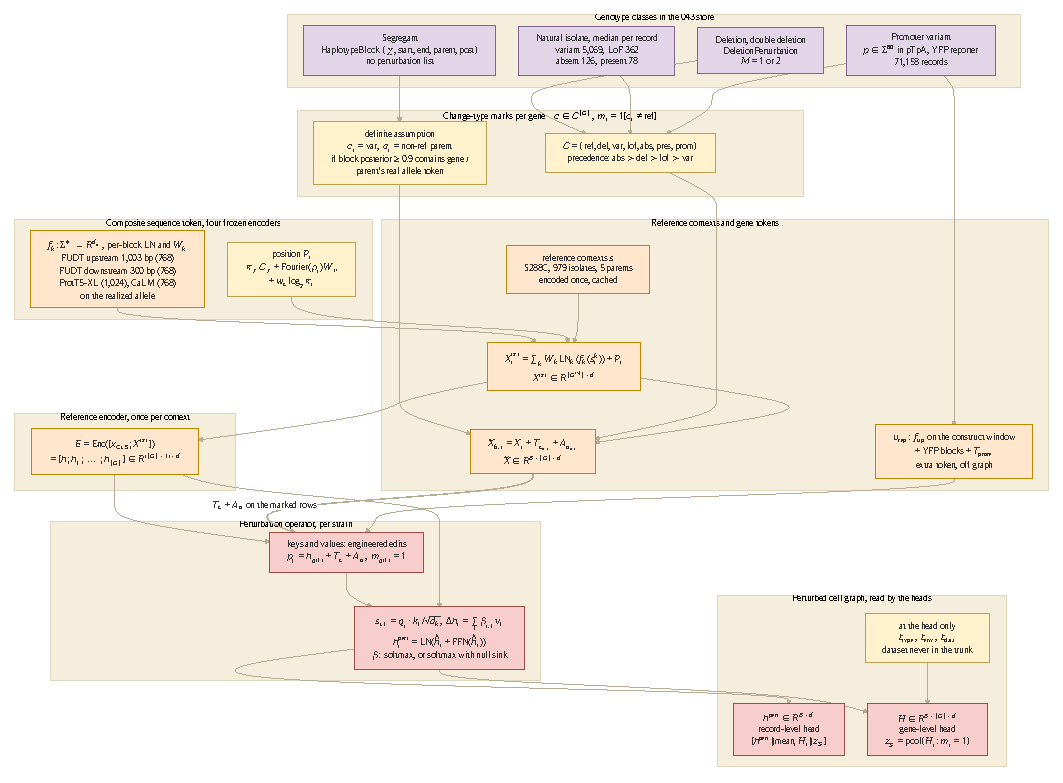
\includegraphics[width=\linewidth,height=0.87\textwidth,keepaspectratio]{figures/mermaid-input-side.pdf}\par\vspace{2pt}
\caption[]{\textbf{Every genotype class reaches the perturbation operator through one
composite sequence token per gene and one encoder pass per reference context.} Top, the
genotype classes and their change-type marks; middle, the four frozen sequence encoders
and the position term, the reference contexts (S288C, each isolate, each non-BY parent)
and their gene tokens, the realized tokens and the reporter token, whose promoter block is
the same FUDT upstream encoder on the construct window; the encoder runs once per context
and is cached; bottom, the operator over the engineered edits and the perturbed states the
heads read, where the type, environment and dataset tokens enter.}
\label{fig:input-side}
\end{figure}
\end{landscape}
%% Generated by notes/assets/publish/scripts/mermaid_pdf.sh from
%% notes/experiments.043-expression-proteome-morphology.mermaid.input-side.md

\subsection{Owner decisions\secstatus{todo}}
\label{sec:input-decisions}

Each item names the recommended option first, then the alternative and the condition under
which it would win. Table~\ref{tab:decisions} carries the same rows with their measured
facts.

\begin{enumerate}
\item \textbf{Base token.} Composite frozen sequence token, Eq.~\ref{eq:input-composite},
with the position term. Alternatives: nucleotide-transformer windows in place of FUDT, for
a host with no FUDT species token (one yeast arm compares the two families now); ESM2 650M
in place of ProtT5 on cost. The identity table is the transductive-ceiling ablation only.
\item \textbf{Absence and deletion.} Two change types; report the cosine of
$T_{\mathrm{del}}$ and $T_{\mathrm{abs}}$ after training.
\item \textbf{Isolates.} Own reference context, operator carries the engineered edits
only (Sec.~\ref{sec:input-isolates}). Alternative: the interim loss-of-function plus
absence mask with allele tokens, if a first run must precede the per-context encoder
(owner question 1).
\item \textbf{Segregant gene membership.} Whole-gene containment, with the parent's actual
allele token on marked genes; all five non-BY parents are collection members.
\item \textbf{Position.} On for every class, Eq.~\ref{eq:input-position}; isolate-own
coordinates deferred to chromosome-scale assemblies.
\item \textbf{Context tokens.} Allele parent on the gene token; environment and ontology
path read by the head (main) or attended after the operator (arm 1); dataset only as the
per-dataset bias at the head, in every arm.
\item \textbf{Normalization at large $M$.} Moot under the main isolate design; softmax;
the sigmoid gate as an arm for the segregant class alone.
\item \textbf{Accessory ORFs and the reporter.} Encode both as extra tokens from the same
encoders; Vaishnav stays in the plan, its linear evaluations run first, and its joint entry
waits on the Addgene 127546 sequence in the constructs tier (owner question 2).
\end{enumerate}
